
\begin{slide}
\heading{Mutual exclusion using semaphores}

A semaphore that is used to enforce mutual exclusion is initially up.  A
process that enters the critical region does a \SCALA{down}, to block other
processes from entering.  When it leaves the critical region it does an
\SCALA{up}, to allow other processes to proceed.
\end{slide}

%%%%%


\begin{slide}
\heading{Signalling using semaphores}

By contrast a \emph{signalling semaphore} is initially down.  A process can
send a signal by performing an \SCALA{up}.  A process waits for a signal by
performing a \SCALA{down}.
\begin{scala}
private val signal = new Semaphore(false)
def signaller = proc{ ...; signal.up; ... }
def waiter = proc{ ...; signal.down; ... }
\end{scala}  
The \SCALA{waiter} cannot proceed before the signal is sent (but the
\SCALA{signaller} can proceed before the signal is received).

Note that the signal is received by only one other process.  Note also that if
the |signaller| performs the signal before the |waiter| is ready, the signal
is not lost.
\end{slide}

%%%%%

\begin{slide}
\heading{Signalling using semaphores}

Alternatively, the signalling semaphore can be created using
\begin{scala}
private val signal = new SignallingSemaphore
\end{scala}
via the definition
\begin{scala}
class SignallingSemaphore extends Semaphore(false)
\end{scala}
\end{slide}

%%%%%

\begin{slide}
\heading{Semaphores versus conditions}

Semaphores and conditions are similar, in that each provides a signalling
mechanism.

The main difference is that a semaphore has a state: it is either up or down.
This means that if an |up| is performed before a thread is waiting, then the
signal is not lost.  

By contrast, if a signal is performed on a condition when
no thread is waiting, then the signal is lost: in such cases, it is often
appropriate to use the condition in combination with a boolean variable. 
\end{slide}

%%%%%

\begin{slide}
\heading{Synchronising using semaphores}

Two processes can synchronise using a pair of signalling semaphores: each
signals to the other when it reaches the synchronisation point; neither
proceeds until it has received the signal from the other.
\begin{scala}
val signal1 = new SignallingSemaphore
val signal2 = new SignallingSemaphore
def p1 = proc{ ...; signal1.up; signal2.down; ... }
def p2 = proc{ ...; signal2.up; signal1.down; ... }
\end{scala}
\end{slide}

%%%%%

\begin{slide}
\heading{Synchronising using semaphores}

The code on the previous slide works fine if the threads use the semaphores to
synchronise just once.  However, it can go wrong if the threads use the same
semaphores to synchronise multiple times. 
%
\begin{scala}
def p1 = proc{ for(i <- 1 to 2){ ...; signal1.up; signal2.down; ... } }
def p2 = proc{ for(i <- 1 to 2){ ...; signal2.up; signal1.down; ... } }
\end{scala}
%
%% Consider an execution of the above where each thread should executes the loop
%% precisely twice.
The following sequence of events is possible, where the
subscripts represent the iteration number.
\[
\begin{align}
\sm{signal1.up}_1,\; \sm{signal2.up}_1,\; \sm{signal2.down}_1,\;
   \sm{signal1.up}_2
\end{align}
\]
Thread~|p2| is suspended after performing its first signal, so that |p1|
performs its second signal \emph{before} |p2| consumes the first signal. 
With our implementation of semaphores, the precondition of |up| is not
satisfied, and an exception is thrown. 
\end{slide}

%%%%%

\begin{slide}
\heading{Synchronising using semaphores}

If we had allowed an |up| when the semaphore is already up (and made it a
no-op), the execution would have continued something like:
\[
\begin{align}
\sm{signal1.up}_1,\; \sm{signal2.up}_1,\; \sm{signal2.down}_1,\;
   \sm{signal1.up}_2, \\
\sm{signal1.down}_1,\; \sm{signal2.up}_2,\; \sm{signal2.down}_2
\end{align}
\]
Here the second signal by |p1| is lost.  Subsequently, |p1| terminates, but
|p2| is stuck waiting for a second signal.
\end{slide}

%%%%%

\begin{slide}
\heading{Synchronising using semaphores}

A solution is to reverse the order of events in one of the threads.
\begin{scala}
def p1 = proc{ for(...){ ...; signal1.up; signal2.down; ... } }
def p2 = proc{ for(...){ ...; signal1.down; signal2.up; ... } }
\end{scala}
%
We can reason as follows (recall the ``happens before'' relation $\prec$).
\[
\begin{array}{rcl@{\qquad}l}
\sm{signal1.up}_1 & \prec & \sm{signal1.down}_1 & 
  \mbox{(signal on {\scalashape signal1})} \\
 & \prec & \sm{signal2.up}_1 & \mbox{(program order for \SCALA{p2})} \\
 & \prec & \sm{signal2.down}_1 & \mbox{(signal on {\scalashape signal2})} \\
 & \prec & \sm{signal1.up}_2 & \mbox{(program order for \SCALA{p1})} \\
 & \prec & \ldots
\end{array}
\]
In particular, the events happen in the expected order, and neither thread
completes the synchronisation on the $n$th iteration before the other thread
has signalled on that iteration.
%
The precondition of |up| is satisfied since $\sm{signal1.down}_n \prec
\sm{signal1.up}_{n+1}$, for each~$n$, and similarly for |signal2|.
\end{slide}

%%%%%

\begin{slide}
\heading{Example: a partial queue using semaphores}

We will implement a partial queue using semaphores.  

If a |dequeue| finds that the queue is empty, it will wait for a signal on a
signalling semaphore |dequeueWait|.  When a subsequent |enqueue| signals on
this semaphore, it will indicate that the queue is now non-empty (in fact,
that the queue contains precisely one element), and the dequeue can proceed.

In addition, we have to protect the shared variables from race conditions.  We
will use a |MutexSemaphore| for this. 

When an |enqueue| finishes, it will either signal on |dequeueWait| to a
waiting |dequeue| if there is one (and leave the mutex down), or lift the
mutex.  We record the number of waiting |dequeues| to support this.
\end{slide}

%%%%%

\begin{slide}
\heading{Example: a partial queue using semaphores}

\begin{scala}
class SemaphorePartialQueue[T] extends PartialQueue[T]{
  /** The queue itself. */
  private val queue = new scala.collection.mutable.Queue[T]

  /** Number of waiting dequeues. */
  private var waitingDequeues = 0

  /** Semaphore to provide mutual exclusion. */
  private val mutex = new MutexSemaphore

  /** Semaphore on which a dequeue waits until the queue is non-empty. */
  private val dequeueWait = new SignallingSemaphore

  // Invariant: if waitingDequeues > 0 and mutex is up, then the queue is empty.
  ...
}
\end{scala}
\end{slide}

%%%%%

\begin{slide}
\heading{Example: a partial queue using semaphores}

\begin{scala}
  def enqueue(x: T) = {
    mutex.down
    queue.enqueue(x)
    if(waitingDequeues > 0) dequeueWait.up // pass the baton to a dequeue at (1)
    else mutex.up
  }

  def dequeue: T = {
    mutex.down
    if(queue.isEmpty){  // have to wait
      waitingDequeues += 1; mutex.up
      dequeueWait.down                         // wait for signal (1)
      assert(queue.length == 1)
      waitingDequeues -= 1
    }
    val result = queue.dequeue; mutex.up; result
  }
\end{scala}
\end{slide}

%%%%%

\begin{slide}
\heading{Passing the baton}

The technique used by |enqueue| is known as \emph{passing the baton}.  It
decides what sort of operation should run next ---either a waiting dequeue or
a new operation--- and ``passes it the baton'' by lifting the appropriate
semaphore. 

Note that when a thread passes the baton to a thread waiting on a signalling
semaphore, it leaves the mutex semaphore down: the latter takes over the
rights implied by possession of the mutex.  

By contrast, the waiting thread should lift the mutex before waiting,
otherwise the system will deadlock.

The technique of passing the baton is quite generally applicable.  Often the
current thread is in the best position to decide which thread can run next.
\end{slide}

%%%%%


\begin{slide}
\heading{Barrier synchronisation}

Recall that a barrier synchronisation can be used to synchronise $n>1$
processes.  Each process in turn calls \SCALA{sync} on the barrier.  Once all
$n$ processes have called \SCALA{sync}, the processes can continue.
%% \end{slide}

%% %%%%%

%% \begin{slide}
%% \heading{Barrier synchronisation}

We define a class
\begin{scala}
class Barrier(n: Int){ def sync = { ... } }
\end{scala}%
%
to implement barrier synchronisation.  

We keep track of the number of threads currently waiting in a variable
\SCALA{waiting}.  We protect this using a mutex semaphore. 

We use a signalling semaphore \SCALA{waitSem} to block the first $n-1$
threads.  The $n$th thread signals on this semaphore to unblock
another thread, i.e.~passes it the baton.  That thread passes the
baton to another waiting thread (assuming $n \ge 3$), and so on.  The
final thread to be awoken raises the mutex, to pass the baton to a
thread on the next round.
\end{slide}


%%%%%

\begin{slide}
\heading{Barrier synchronisation}

\begin{scala}
class Barrier(n: Int){
  private var waiting = 0 // # processes waiting
  private val waitSem = new SignallingSemaphore
  private val mutex = new MutexSemaphore

  def sync = {
    mutex.down
    if(waiting == n-1) waitSem.up // start the waking up
    else{ 
      waiting += 1; mutex.up; waitSem.down  // wait until woken
      waiting -= 1
      if(waiting > 0) waitSem.up // pass baton to next waiting thread
      else mutex.up // pass baton to thread on next round.
    }
  }
}
\end{scala}

\end{slide}

%%%%%
\begin{slide}
\heading{Barrier synchronization}

\begin{itemize}
\item
The first $n-1$ processes  end up blocked on \SCALA{waitSem.down};

\item The $n$th process performs \SCALA{waitSem.up}, to pass the baton to
another thread, and returns;

\item In turn, $n-2$ threads are woken, decrement \SCALA{waiting}, and wake up
the next thread;

\item The final thread to be woken, performs \SCALA{mutex.up} to allow the
following round of synchronisation to proceed.
\end{itemize}

Note that after the $n$th process has called |sync|, no other thread can pass
the mutex until the last thread exits, since \SCALA{mutex} remains down.
This prevents different rounds from interfering.
\end{slide}

%%%%%

% \begin{slide}
% \heading{Passing the baton}

% The implementation of the barrier synchronisation illustrates a technique
% known as \emph{passing the baton}: each process ``passes the baton'' to
% another process to allow it to continue.
% %
% \begin{itemize}
% \item
% During the first stage, while \SCALA{waiting < n}, each process passes the
% baton to a process that's starting (or yet to start) the \SCALA{sync} method,
% by performing \SCALA{mutex.up}.

% \item
% The $n$th process passes the baton to one of the processes waiting on
% \SCALA{waitSem}, by performing the \SCALA{waitSem.up}.

% \item
% The next $n-2$ processes to leave pass the baton to another processes waiting
% on \SCALA{waitSem}, by performing the \SCALA{waitSem.up}.

% \item
% The last process to leave passes the baton to a process that's starting (or yet
% to start) the \SCALA{sync} method, by performing \SCALA{mutex.up}.
% \end{itemize}
% \end{slide}

%%%%%%%%%%

\begin{selfnote}

Note that each awakened process passes the baton to precisely one other
process. 

It's common to have to keep track of how many processes are waiting on a
semaphore in order to decide to whom to pass the baton.
\end{selfnote}

%%%%%%%%%%%%%%%%%%%%%%%%%%%%%%%%%%%%%%%%%%%%%%%%%%%%%%%%%%%%

\begin{slide}
\heading{Example: a synchronous channel}

We will now implement a synchronous channel (suitable for use by multiple
senders and receivers) using semaphores.  We will need three signals for each
message, in the following order:
%
\begin{enumerate}
\item The sender will signal to the receiver that it has deposited a value, on
  semaphore |slotFull|.

\item The receiver will signal back to the sender on semaphore |continue|,
  thereby providing a synchronisation.

\item The sender will signal to the sender on the next round that the slot has
  been emptied, on semaphore |slotEmptied|.
\end{enumerate}
%
These three semaphores will collectively provide mutual exclusion.
\end{slide}

%%%%%

\begin{slide}
\heading{Example: a synchronous channel}

\begin{center}
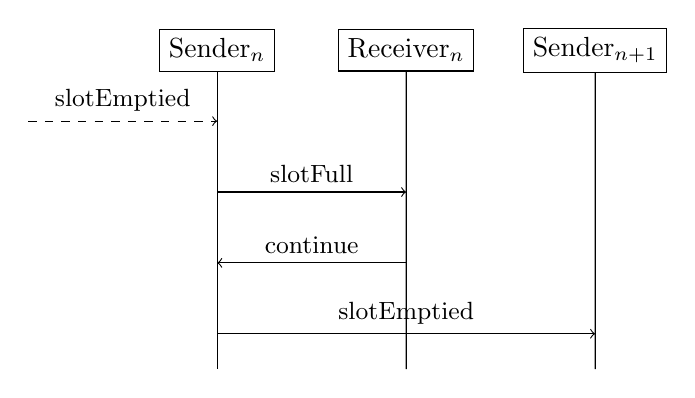
\begin{tikzpicture}[xscale = 1.2,yscale = 0.9]
\draw (0,0) node[draw](sender){ \scalacolour Sender$_n$ };
\draw (2,0) node[draw](receiver){ \scalacolour Receiver$_n$ };
\draw (4,0) node[draw](sender2){ \scalacolour Sender$_{n+1}$ };
\draw (sender) -- ++ (0,-4.5);
\draw (receiver) -- ++ (0,-4.5);
\draw (sender2) -- ++ (0,-4.5);
\draw[->,dashed] (-2,-1) -- node[above] {\small\scalastyle slotEmptied} (0,-1);
\draw[->] (0,-2) -- node[above] { \small\scalastyle slotFull} (2,-2);
\draw[<-] (0,-3) -- node[above] { \small\scalastyle continue} (2,-3);
\draw[->] (0,-4) -- node[above] {\small\scalastyle slotEmptied} (4,-4);
\end{tikzpicture}
\end{center}
\end{slide}


%%%%%


\begin{slide}
\heading{Example: a synchronous channel}

\begin{scala}
class SyncChanSemaphores[A] extends SyncChanT[A]{  
  /** The current or previous value. */
  private var value = null.asInstanceOf[A]

  /** A semaphore for signalling to receiver that a value has been deposited. */
  private val slotFull = new SignallingSemaphore

  /** A semaphore for signalling to current sender that it can continue. */
  private val continue = new SignallingSemaphore

  /** A semaphore for signalling to the next sender that the previous value has
    * been read. */
  private val slotEmptied = new MutexSemaphore
  ...
}
\end{scala}
\end{slide}

%%%%%

\begin{slide}
\heading{Example: a synchronous channel}

The three semaphores will collectively provide mutual exclusion: when any
thread is active, all semaphores will be down; when no thread is active, a
single semaphore will be up.  Initially, just |slotEmptied| is up.

There is no need to have an extra |full| variable indicating that the current
value is valid: the |slotFull| and |slotEmptied| semaphores fulfil that role. 
\end{slide}

%%%%%

\begin{slide}
\heading{Example: a synchronous channel}

\begin{scala}
  def send(x: A) = {
    slotEmptied.down       // wait for previous value to be consumed (3)
    value = x               // deposit my value
    slotFull.up             // pass baton to receiver at (1)
    continue.down           // wait for receiver (2)
    slotEmptied.up          // pass baton to next sender at (3)
  }

  def receive: A = {
    slotFull.down           // wait for sender (1)
    val result = value      // take value
    continue.up             // pass baton to current sender at (2)
    result
  }
\end{scala}
\end{slide}

%%%%%

\begin{slide}
\heading{Example: a synchronous channel}

The signals must happen in the expected order:
\[
\begin{array}{rcl@{\qquad}l}
\sm{slotEmptied.down}_1 & \prec & \sm{slotFull.up}_1 & 
  \mbox{(program order for \SCALA{send})} \\
  & \prec & \sm{slotFull.down}_1 & \sm{(signal on {\scalashape slotFull})} \\
  & \prec & \sm{continue.up}_1 & \mbox{(program order for \SCALA{receive})} \\
  & \prec & \sm{continue.down}_1 & \sm{(signal on {\scalashape continue})} \\
  & \prec & \sm{slotEmptied.up}_1 & \mbox{(program order for \SCALA{send})} \\
  & \prec & \sm{slotEmptied.down}_2 & 
     \sm{(signal on {\scalashape slotEmptied})} \\
  & \prec & \ldots
\end{array}
\]

In particular, for each semaphore $s$,\, $s.\sm{down}_n \prec
s.\sm{up}_{n+1}$, so no signal is lost.
\end{slide}

%%%%%

\begin{slide}
\heading{Example: a synchronous channel}

Here's an incorrect version, where |receive| (rather than |send|) signals on
|slotEmptied|. 
%
\begin{scala}
  def send(x: A) = {
    slotEmptied.down       // wait for previous value to be consumed (3)
    value = x               // deposit my value
    slotFull.up             // pass baton to receiver (1)
    continue.down           // wait for receiver (2)
  }

  def receive: A = {
    slotFull.down           // wait for sender (1)
    val result = value      // take value
    continue.up             // pass baton to current sender (2)
    slotEmptied.up          // pass baton to next sender at (3)
    result
  }
\end{scala}
\end{slide}

%%%%%

\begin{slide}
\heading{Example: a synchronous channel}

With the version on the previous slide, suppose a |send| is suspended just
before performing |continue.down|.  Then the current receiver can signal on
|continue| and |slotEmptied|.  Then the following sender and receiver can run,
leading to a second |continue.up|, which breaks the precondition of |up|.  If
our implementation of semaphores had allowed such a second |up|, it would have
been a lost signal.
\end{slide}

%%%%%%%%%%%%%%%%%%%%%%%%%%%%%%%%%%%%%%%%%%%%%%%%%%%%%%%

\begin{slide}
\heading{Example: first-come-first-served mutual exclusion}

Consider a mechanism to allow clients to access a shared resource
under mutual exclusion.  Suppose we also want to ensure that clients
gain access in a first-come-first-served order.  (Note that this will have a
performance overhead, but might be desirable in some circumstances.)
%
We will implement this using semaphores. 

If a process is forced to wait to access the resource, it will create a new
semaphore, place it in a queue, and then wait on it.  When a process finishes
with the resource, it will pass the baton to the process waiting on the first
semaphore in the queue (if there is one) by raising that semaphore.

We also need to record whether the resource is currently being used.  

And we need a semaphore to enforce mutual exclusion on the object's variables.
\end{slide}

%%%%%% 

\begin{slide}
\heading{Example: first-come-first-served mutual exclusion}

\begin{scala}
class MutexQueue{
  /** A queue of semaphores for waiting threads. */
  private val queue = new scala.collection.mutable.Queue[Semaphore]

  /** Is the resource busy? */
  private var busy = false

  /** Semaphore for mutual exclusion on this object's variables. */
  private val mutex = new MutexSemaphore

  // Invariant: if the mutex is up, and busy = false, then queue is empty.
  ...
}
\end{scala}
\end{slide}

%%%%%

\begin{slide}
\heading{Example: first-come-first-served mutual exclusion}

\begin{scala}
  def enter = {
    mutex.down
    if(busy){ // have to wait
      val sem = new SignallingSemaphore; queue.enqueue(sem)
      mutex.up; sem.down                  // wait turn (1)
    }
    else assert(queue.isEmpty)
    busy = true; mutex.up
  }

  def leave = {
    mutex.down; busy = false
    if(queue.nonEmpty){                 // wake up next process at (1)
      val first = queue.dequeue; first.up
    }
    else mutex.up
  }
\end{scala}
\end{slide}

%%%%%

\begin{slide}
\heading{Selective passing the baton}

This technique can be used in a number of scenarios to allow the current
thread to selectively pass the baton to a particular thread: each thread that
has to wait, creates a new semaphore, stores it, and waits on it.

Sometimes it is necessary to store some extra information with each such
semaphore, so that the current thread can choose between the waiting threads.
This choice should be made so that the thread that receives the signal can
then do something useful. 
\end{slide}
